\documentclass[11pt,a4paper]{article}
\usepackage[T1]{fontenc}
\usepackage[utf8]{inputenc}
\usepackage{lmodern}
\usepackage{amsmath,amssymb}
\usepackage{geometry}
\usepackage{microtype}
\usepackage{parskip}
\usepackage{titlesec}
\usepackage{tikz}
\usetikzlibrary{positioning}

\geometry{top=2.5cm, bottom=2.5cm, left=2.8cm, right=2.8cm}
\titlespacing*{\section}{0pt}{1.6ex}{0.6ex}
\setlength{\parskip}{5pt}

\newcommand{\hb}{H_b}

\begin{document}

\begin{center}
{\large\textbf{EE 533 -- Assignment 3}} \quad Kerem Recep Gür \quad 2448462
\end{center}
\medskip\hrule\bigskip

%-----------------------------------------------------------------------
\section*{Problem 1 \normalfont\small(5.38)}

Probabilities in decreasing order:
$p = \bigl(\tfrac{6}{25}, \tfrac{6}{25}, \tfrac{4}{25}, \tfrac{4}{25},
\tfrac{3}{25}, \tfrac{2}{25}\bigr)$, labelled $a$ through $f$.

\medskip
\textbf{(a) $D=2$.}

Combine the two smallest at each step (combined node shown in brackets):

\[
\begin{array}{ll}
\text{Step 1:} & e(3/25)+f(2/25)\to [ef](5/25)\\
\text{Step 2:} & c(4/25)+d(4/25)\to [cd](8/25)\\
\text{Step 3:} & b(6/25)+[ef](5/25)\to [bef](11/25)\\
\text{Step 4:} & a(6/25)+[cd](8/25)\to [acd](14/25)\\
\text{Step 5:} & [acd](14/25)+[bef](11/25)\to \text{root}
\end{array}
\]

Reading back from the tree (0 = left, 1 = right):

\[
\begin{array}{c|c|c}
\text{Symbol} & \text{Prob} & \text{Codeword}\\\hline
a & 6/25 & 00 \\
b & 6/25 & 10 \\
c & 4/25 & 010 \\
d & 4/25 & 011 \\
e & 3/25 & 110 \\
f & 2/25 & 111
\end{array}
\]

Expected word length:
\[
\bar{L} = \frac{2(6)+2(6)+3(4)+3(4)+3(3)+3(2)}{25}
= \frac{12+12+12+12+9+6}{25} = \frac{63}{25} = 2.52 \text{ bits}.
\]

\medskip
\textbf{(b) $D=4$.}

For 4-ary Huffman with $n=6$ symbols we need $(n-1)\bmod(D-1)=5\bmod 3=2\neq 0$,
so we add $3-2=1$ dummy symbol (prob 0) to make $n=7$.

\[
\begin{array}{ll}
\text{Step 1:} & \text{Combine 4 smallest: }d(4/25),\,e(3/25),\,f(2/25),\,\text{dummy}(0)\to [def\cdot](9/25)\\
\text{Step 2:} & \text{Combine remaining 4: }[def\cdot](9/25),\,a(6/25),\,b(6/25),\,c(4/25)\to\text{root}
\end{array}
\]

Assigning digits 0--3 at each branch:

\[
\begin{array}{c|c|c}
\text{Symbol} & \text{Prob} & \text{Codeword}\\\hline
a & 6/25 & 1 \\
b & 6/25 & 2 \\
c & 4/25 & 3 \\
d & 4/25 & 00 \\
e & 3/25 & 01 \\
f & 2/25 & 02
\end{array}
\]

Expected word length (in 4-ary digits):
\[
\bar{L} = \frac{1(6)+1(6)+1(4)+2(4)+2(3)+2(2)}{25}
= \frac{6+6+4+8+6+4}{25} = \frac{34}{25} = 1.36.
\]

%-----------------------------------------------------------------------
\section*{Problem 2 \normalfont\small(5.39)}

$C:X\to\{0,1\}^*$ is nonsingular (injective) but not uniquely decodable.

\textbf{(a) Compare $H(C(X))$ to $H(X)$.}

Since $C$ is nonsingular, distinct values of $X$ map to distinct codewords,
so $C(X)$ determines $X$ uniquely.
$C(X)$ is a bijective function of $X$, therefore
\[
  H(C(X)) = H(X).
\]

\textbf{(b) Compare $H(C(X^n))$ to $H(X^n)$.}

$C(X^n)$ denotes the concatenation $C(X_1)C(X_2)\cdots C(X_n)$.
Since $C$ is not uniquely decodable, two different sequences $x^n\neq \tilde{x}^n$
can produce the same concatenation.  The mapping $x^n\mapsto C(X^n)$ is
therefore many-to-one, so
\[
  H(C(X^n)) < H(X^n).
\]

%-----------------------------------------------------------------------
\section*{Problem 3 \normalfont\small(15.8)}

The general Slepian--Wolf region for $(X,Y)$ is
\[
R_X \ge H(X\mid Y),\quad
R_Y \ge H(Y\mid X),\quad
R_X+R_Y \ge H(X,Y).
\]
When $Y=f(X)$:
\[
H(Y\mid X)=0,\qquad H(X,Y)=H(X),\qquad H(X\mid Y)=H(X\mid f(X)).
\]
Denote $H(X\mid f(X))$ as $\alpha$ and $H(f(X))$ as $\beta$, so $\alpha+\beta=H(X)$.
The region simplifies to:
\[
  R_X \ge \alpha,\qquad R_Y \ge 0,\qquad R_X+R_Y\ge H(X).
\]

\begin{center}
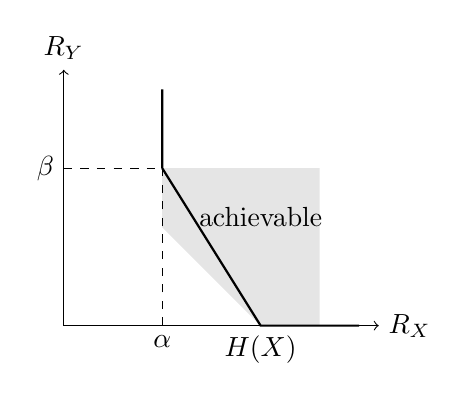
\begin{tikzpicture}[scale=2.5]
  \draw[->] (0,0) -- (1.6,0) node[right] {$R_X$};
  \draw[->] (0,0) -- (0,1.3) node[above] {$R_Y$};
  % shaded achievable region
  \fill[gray!20]
    (0.5,0.8) -- (1.3,0.8) -- (1.3,0) -- (1.0,0) -- (0.5,0.5) -- cycle;
  \draw[thick]
    (0.5,0.8) -- (0.5,1.2)
    (0.5,0.8) -- (1.0,0)
    -- (1.5,0);
  \draw[dashed] (0.5,0) -- (0.5,0.8) node[midway,right] {};
  \draw[dashed] (0,0.8) -- (0.5,0.8);
  \node[below] at (0.5,0) {$\alpha$};
  \node[below] at (1.0,0) {$H(X)$};
  \node[left]  at (0,0.8) {$\beta$};
  \node at (1.0,0.55) {achievable};
\end{tikzpicture}
\end{center}

The region is bounded below by $R_Y=0$, on the left by $R_X=\alpha=H(X\mid f(X))$,
and on the diagonal by $R_X+R_Y=H(X)$.
The corner point is $(\alpha,\,\beta)=\bigl(H(X\mid f(X)),\,H(f(X))\bigr)$.

%-----------------------------------------------------------------------
\section*{Problem 4 \normalfont\small(15.22)}

$Z_1\sim\mathrm{Bern}(p_1)$, $Z_2\sim\mathrm{Bern}(p_2)$ independent;
$X=Z_1+Z_2$, $Y=Z_1-Z_2$.

Since $(X,Y)\leftrightarrow(Z_1,Z_2)$ is a bijection
($Z_1=(X{+}Y)/2$, $Z_2=(X{-}Y)/2$):
\[
  H(X,Y) = H(Z_1,Z_2) = H(p_1)+H(p_2).
\]

For $H(Y\mid X)$: given $X{=}0$ or $X{=}2$, $Y$ is determined ($Y=0$).
Given $X{=}1$, $Y=\pm 1$ with $P(Y{=}1\mid X{=}1)=\frac{p_1(1-p_2)}{p_1(1-p_2)+(1-p_1)p_2}$.
Denote $q=\frac{p_1(1-p_2)}{p_1(1-p_2)+(1-p_1)p_2}$.  Then:
\[
  H(Y\mid X) = \bigl[p_1(1-p_2)+(1-p_1)p_2\bigr]\,h(q),
\]
where $h(\cdot)$ is the binary entropy function.

By symmetry (swapping $+$ and $-$):
\[
  H(X\mid Y) = \bigl[p_1 p_2+(1-p_1)(1-p_2)\bigr]\,h\!\left(\frac{p_1 p_2}{p_1 p_2+(1-p_1)(1-p_2)}\right).
\]

\textbf{(a)} The Slepian--Wolf rate region for $(R_X,R_Y)$:
\[
  R_X \ge H(X\mid Y),\quad
  R_Y \ge H(Y\mid X),\quad
  R_X+R_Y \ge H(p_1)+H(p_2).
\]

\textbf{(b)} For $(Z_1,Z_2)$: since $Z_1\perp Z_2$,
$H(Z_1\mid Z_2)=H(p_1)$ and $H(Z_2\mid Z_1)=H(p_2)$, so the Slepian--Wolf region is simply
\[
  R_{Z_1}\ge H(p_1),\quad R_{Z_2}\ge H(p_2),
\]
a single corner point (no rate tradeoff possible).

For $(X,Y)$: $H(X\mid Y)<H(p_1)+H(p_2)$ and $H(Y\mid X)<H(p_1)+H(p_2)$,
so both encoders can reduce their individual rates by exploiting the
correlation.  The $(X,Y)$ region strictly contains the $(Z_1,Z_2)$ region
and allows a nontrivial sum-rate tradeoff along the diagonal $R_X+R_Y=H(p_1)+H(p_2)$.

%-----------------------------------------------------------------------
\section*{Problem 5 \normalfont\small(15.24)}

$Z_1,Z_2,Z_3$ i.i.d.\ $\mathrm{Bern}(p)$;
$X_1=Z_1$, $X_2=Z_1+Z_2$, $X_3=Z_1+Z_2+Z_3$.

Since $(X_1,X_2,X_3)\leftrightarrow(Z_1,Z_2,Z_3)$ is a bijection
($Z_1=X_1$, $Z_2=X_2-X_1$, $Z_3=X_3-X_2$):
\[
  H(X_1,X_2,X_3)=3H(p).
\]

\textbf{Conditional entropies:}
\begin{align*}
H(X_1\mid X_2,X_3) &= H(Z_1\mid Z_1{+}Z_2,\;Z_1{+}Z_2{+}Z_3)
  = H(Z_1\mid Z_1{+}Z_2) = 2p(1-p),\\
  &\quad\text{(given }X_2\text{ and }X_3\text{, }Z_3=X_3-X_2\text{ is known; remaining uncertainty = }H(Z_1|Z_1{+}Z_2))\\[4pt]
H(X_2\mid X_1,X_3) &= H(Z_2\mid Z_2{+}Z_3) = 2p(1-p),\\[4pt]
H(X_3\mid X_1,X_2) &= H(Z_3) = H(p).
\end{align*}

\textbf{Pair conditional entropies:}
\begin{align*}
H(X_1,X_2\mid X_3) &= H(Z_1,Z_2\mid Z_1{+}Z_2{+}Z_3)
  = 3H(p)-H(S_3),\\
H(X_1,X_3\mid X_2) &= H(Z_1,Z_3\mid Z_1{+}Z_2)
  = H(Z_1\mid Z_1{+}Z_2)+H(Z_3) = 2p(1-p)+H(p),\\
H(X_2,X_3\mid X_1) &= H(Z_2,Z_3) = 2H(p).
\end{align*}
where $S_3=Z_1+Z_2+Z_3\sim\mathrm{Binomial}(3,p)$ with
$H(S_3)=-(1-p)^3\log(1-p)^3-3p(1-p)^2\log 3p(1-p)^2
        -3p^2(1-p)\log 3p^2(1-p)-p^3\log p^3$.

\textbf{Slepian--Wolf rate region:}
\[
\begin{aligned}
R_1 &\ge 2p(1-p), \\
R_2 &\ge 2p(1-p), \\
R_3 &\ge H(p), \\
R_1+R_2 &\ge 3H(p)-H(S_3), \\
R_1+R_3 &\ge 2p(1-p)+H(p), \\
R_2+R_3 &\ge 2H(p), \\
R_1+R_2+R_3 &\ge 3H(p).
\end{aligned}
\]

\end{document}
